\chapter{\label{chapter:PropagatorStates}The State Vector and State Management}
\chapauthor{Darrel J. Conway}{Thinking Systems, Inc.}

GMAT supplies a class, the GmatState, which provides a low level container for mission related
state information manipulated by the system during a simulation.  The GmatState is populated with
data from the objects in GMAT's current model so that the code that implements the processes in the
simulation can act on the data in a generic fashion.  The synchronization between the data that
is manipulated and the objects that supply these data is handled by classes derived from the
StateManager class.  These interactions are described at a high level in this chapter.  Specific
uses of the state vector and manager can be found in teh chapters describing propagation
(Chapter~\ref{chapter:PropagatorOverview}) and orbit determination
(Chapter~\ref{chapter:Estimation}).

\section{Design Motivation and Overview}

The combination of one or more GmatState objects and one or more associated StateManagers as
implemented in GMAT follows the Mediator design pattern.  The GmatState acts as an intermediary
between the objects in the model and the algorithms that access and manipulate the data associated
with those objects.

You can see an example of this mediation in GMAT's propagation subsystem.  Consider a mission
consisting of two spacecraft that are propagated for a day using a Runge-Kutta integrator and a
force model consisting of a 4x4 geopotential model, point mass effects from the Sun and Moon, solar
radiation pressure, and atmospheric drag modeled using the MSISE-90 atmosphere model.  In GMAT, the
user configures four objects to model this system: two spacecraft, an ODEModel that holds the force
model, and a Runge-Kutta integrator.  The mission control sequence that uses these objects is a
single Propagate command.  Ignoring the details of the object configuration, the setup for this
mission can be scripted:

\begin{quote}
\texttt{Create Spacecraft sat1 sat2\\
\\
Create ForceModel fm\\
Create Propagator prop\\
prop.FM = fm\\
\\
Propagate prop(sat1, sat2) {sat1.ElapsedDays = 1.0}}
\end{quote}

\noindent GMAT collects the integrator and force model in a container called a PropSetup (see
Section~\ref{section:PropSetup}).  GMAT's PropSetup class has a member pointer for a Propagator and
a second pointer for an ODEModel.  Each PropSetup also has a StateManager member -- in the case of
propagation, the StateManager is an instance of the PropagationStateManager class -- that
communicates with the other objects in the system to retrieve the values of the data that needs to
be propagated and arranges those data into a single vector that the force model and integrator
understand. GMAT's propagation subsystem -- that is, the integrator and associated ODEModel -- use
this data vector and an associated mapping of ordinary differential equations to calculate a new
vector of numbers at some different time.  In other words, GMAT's propagation subsystem has minimal
knowledge of the objects that are being propagated.  At the level of the evolution algorithm, the
propagation subsystem merely maps a vector of numbers at some epoch into a new vector of number at
some other epoch.  The propagation state manager associated with the PropSetup container handles
the communications of that vector numbers with the corresponding data in the objects.

Returning to our example, when the scripting listed above is built, GMAT constructs two spacecraft
named sat1 and sat2.  These spacecraft are added to GMAT's configuration.  Next GMAT creates an
ODEModel named fm and adds it to the configuration.  Then GMAT creates a PropSetup named prop and
 adds it to the configuration\footnote{The command ``Create Propagator prop'' uses GMAT's factories
to build a PropSetup container named prop.}.  The PropSetup, prop, includes a member instance of the
PropagationStateManager class, and two pointers: a pointer to a Propagator object and a pointer to
an ODEModel object, both initialized to NULL.  The object configuration lines, omitted in this
example, populate the Propagator side of that PropSetup.  Finally, the line ``prop.FM = fm''
assigns the ODEModel named fm to the PropSetup.  This object creation and configuration is stored
in GMAT's configuration for use during a run.

The Propagate command is treated similarly.  An instance of teh Proapgate command is created using
GMAT's factory subsystem and then placed in the Mission Control Sequence.  The command is passed
the string that was used to consttruct it, and that string is decompoed into its constituent
elements.  Once that phase is complete, the Propagate command has strings defining the PropSetup
used for propagation, the names of the objects that need to be propagated, and strings defining the
condition or conditions that terminate propagation.  In our example, the Propagate instance has a
single string defining the PropSetup it uses, ``prop'', a StringArray defining the objects that are
propagated using that PropSetup -- ``sat1'' and ``sat2'' -- and strings identifying the object used
to determine when to stop -- ``sat1'' -- the type of condition that terminates propagation --
``ElapsedDays'' -- and the value that that condition should have when it propagation ends
--~``1.0''.

%\section{\label{section:MissionStateOverview}The Mission State}

% The current values of spacecraft data, the state transition matrix, and other elements that evolve
% in GMAT's model are held, in the propagation subsystem, in the mission state\footnote{Here -- and
% throughout this chapter -- the term ``mission state'' and the word ``state'' represent this
% collection of data elements, unless otherwise specified.  Other chapters in the architectural
% specification may use the word ``state'' for different purposes -- for example, the Solver classes
% all function through finite state machines, where the current location of the system in the
% solution process is assigned a specific status, called a state, and move from one of these
% enumerated stated to another as the solution process is executed.}.  GMAT's mission state can be
% further decomposed into static components, components that evolve through numerical integration,
% components that have analytic evolution operators, and components that are modeled over time using
% stochastic models.
%
% \section{Classes Supporting the Mission State}
%
% The mission state data is culled from the objects that make use of the data contained in the
%state,
% and passed into the elements that the propagators use to calculate the state evolution.  As an
% example, each Spacecraft object manages data representing the position and velocity of that
% particular Spacecraft.  When GMAT needs to model the motion of that spacecraft, it gathers the
% epoch and corresponding position and velocity information in a mission state, and passes that
% mission state to the evolution operator so that the motion associated with the change of epoch can
% be calculated.  A more complete example of this process is presented in
% Section~\ref{section:IntegratorExample}.

\section{The MissionState Class}

% The MissionState class plays two roles in GMAT.  It acts as a container class that takes pointers
% to the objects that supply state data, providing a central location for the state data for mission
% elements that use it.  It also supplies the accumulated state data to those elements in the form
% that they need in order to process it and take actions, and routes any resulting changes in state
% to the objects that receive those changes.
%
% The MissionState class collects data into vectors used by the propagators.  These vectors are
% constructed based on the needs of the propagator, and
%
% GMAT's Numerical Integrators

\subsection{Enumerations used in the MissionState}

The MissionState uses several enumerations used to identify propagation components efficiently.
This section describes each of these enumerations.

\paragraph{PropMode}  The PropMode enumeration identifies the type of propagation used with a given
set of state elements.

\begin{itemize}
\item \textbf{ANALYTIC\_PROP}
\item \textbf{INTEGRATE}
\item \textbf{PRECALCULATED\_PROP}
\end{itemize}

\paragraph{ElementType}  The ElementType enumeration identifies the kind of component contained in
a PropVector

\begin{itemize}
\item \textbf{CARTESIAN\_START}
\item \textbf{CARTESIAN}
\item \textbf{EQUINOCTIAL\_START}
\item \textbf{EQUINOCTIAL}
\item \textbf{STM\_START}
\item \textbf{STM}
\item \textbf{QUARTERNION\_START}
\item \textbf{QUARTERNION}
\item \textbf{MASS}
\item \textbf{USER\_DEFINED}
\item \textbf{UNKNOWN\_ELEMENT\_TYPE}
\end{itemize}

\subsection{MissionState Attributes}

\begin{itemize}
\item\textbf{Real epoch} The epoch of the state data managed by the MissionState.  GMAT requires
that all such state data in a MissionState use the same epoch.
\item\textbf{ObjectArray dataSource} The vector of objects that are propagated
\item\textbf{std::vector<PropMode> propModes} The propagation mode for each object that is
propagated.
\item\textbf{Integer dimension} Total number of elements that are propagated
\item\textbf{PropVector thePropVector} The state data to be propagated
\end{itemize}

\subsubsection{MissionState Methods}

\begin{itemize}
\item\textbf{bool AddSource(GmatBase* src, PropMode mode, ElementType type, Integer elementId)}
Registers an object as a data provider with the MissionState.  The mode parameter identifies the
type of propagation desired: analytic, numerically integrated, or from an ephemeris source.  The
type parameter identified the kind of element that is propagated.  The elementId parameter is the ID
for the start of the data that is propagated.  All propagated data must be accessible using the
generic access methods defined for GmatBase objects, so that the elementId can be used to access
these data.
\item\textbf{bool Initialize()}  Performs preliminary setup of the PropVector prior to propagation.
\item \textbf{bool PrepareToPropagate()}  Completes pre-propagation setup.
\end{itemize}

\section{\label{section:propVector}The PropVector Class}

%The propVector component of the MissionState is a Real array of data sized to match the data vector
%needed by GMAT's numerical integrators for propagation.  The propVector is constructed by the
%MisisonState when the PrepareToPropagate methos if executed by the command that controls the
%propagation.  Figure~\ref{figure:PropVectorComponents} shows a representative layout for a
%propVector.

Figure~\ref{figure:PropVectorComponents} shows a representative layout of the data in a PropVector
for a single spacecraft.  The vector displayed here is the PropVector used by a numerical
integrator that is modeling the evolution of the spacecraft's trajectory, state transition matrix,
and attitude during a finite burn maneuver.  When a MissionState object assembles a PropVector, it
follows a set of ordering rules designed to make the data in the PropVector fall in a specific
order so that access from the propagators is simplified.  The general order, as shown in this
example, is to place trajectory data first in the vector, followed by associated matrices that
evolve along with the trajectory, then attitude data followed by associated attitde matrices, then
user defined elements, and finally transitory elements like mass, which only changes (through
propagation) during maneuvers.

\begin{figure}[htb]
\begin{center}
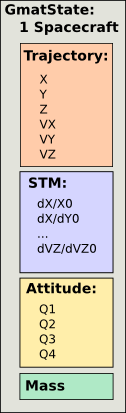
\includegraphics[63,207]{Images/PropVectorComponents.png}
\caption{\label{figure:PropVectorComponents}Representative Elements of a PropVector}
\end{center}
\end{figure}

This ordering can be seen more explicitly in Figure~\ref{figure:ThreeSatPropVector}.  The
PropVector shown in this figure is a vector constructed for three spacecraft, where the mission
needs to propagate the trajectory, state transition matrix, and attitude for all three while
maneuvering all three simultaneously.

\begin{figure}[htb]
\begin{center}
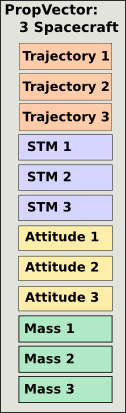
\includegraphics[63,207]{Images/ThreeSatPropVector.png}
\caption{\label{figure:ThreeSatPropVector}Element Arrangement of a PropVector for Three
Spacecraft}
\end{center}
\end{figure}

Figure~\ref{figure:SelectPropVector} shown another example, where the propagation need not
integrate every element of all of the spacecraft.  In this example, the trajector is integrated for
all three spacecraft.  The state transition matrix is only propagated for the first and third
spacecraft, the attitude is propagated for the second, and the first spacecraft is depleting mass
during a maneuver.

\begin{figure}[htb]
\begin{center}
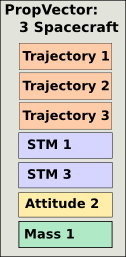
\includegraphics[63,129]{Images/ThreeSatActivePropVector.png}
\caption{\label{figure:SelectPropVector}Three Spacecraft Arrangement for Select
Propagation}
\end{center}
\end{figure}

Figure~\ref{figure:AttitudePropVector} \textbf{This figure needs updating to include the second
PropVector for the trajectory piece} shows a mixed mode propagation, where the trajectory for our
three spacecraft is propagated using a precalculated, ephemeris based propagator and the attitude is
propagated numerically.

\begin{figure}[htb]
\begin{center}
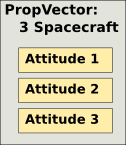
\includegraphics[63,73]{Images/ThreeSatAttitudePropVector.png}
\caption{\label{figure:AttitudePropVector}PropVector for Attitude Only Propagation on Three
Spacecraft}
\end{center}
\end{figure}




